\ifx\wholebook\relax \else
% ------------------------ 

\documentclass{article}
%------------------- Other types of document example ------------------------
%
%\documentclass[twocolumn]{IEEEtran-new}
%\documentclass[12pt,twoside,draft]{IEEEtran}
%\documentstyle[9pt,twocolumn,technote,twoside]{IEEEtran}
%
%-----------------------------------------------------------------------------
%%
% loading packages
%
\newif\ifpdf
\ifx\pdfoutput\undefined % We're not running pdftex
  \pdffalse
\else
  \pdftrue
\fi
%
%
\ifpdf
  \RequirePackage[pdftex,%
            CJKbookmarks,%
       bookmarksnumbered,%
              colorlinks,%
          linkcolor=blue,%
              hyperindex,%
        plainpages=false,%
       pdfstartview=FitH]{hyperref}
\else
  \RequirePackage[dvipdfm,%
             CJKbookmarks,%
        bookmarksnumbered,%
               colorlinks,%
           linkcolor=blue,%
               hyperindex,%
         plainpages=false,%
        pdfstartview=FitH]{hyperref}
  \AtBeginDvi{\special{pdf:tounicode GBK-EUC-UCS2}} % GBK -> Unicode
\fi
\usepackage{hyperref}

% other packages
%-----------------------------------------------------------------------------
\usepackage{graphicx, color}
\usepackage{CJK}
%
% for programming 
%
\usepackage{verbatim}
\usepackage{listings}


\lstdefinelanguage{Smalltalk}{
  morekeywords={self,super,true,false,nil,thisContext}, % This is overkill
  morestring=[d]',
  morecomment=[s]{"}{"},
  alsoletter={\#:},
  escapechar={!},
  literate=
    {BANG}{!}1
    {UNDERSCORE}{\_}1
    {\\st}{Smalltalk}9 % convenience -- in case \st occurs in code
    % {'}{{\textquotesingle}}1 % replaced by upquote=true in \lstset
    {_}{{$\leftarrow$}}1
    {>>>}{{\sep}}1
    {^}{{$\uparrow$}}1
    {~}{{$\sim$}}1
    {-}{{\sf -\hspace{-0.13em}-}}1  % the goal is to make - the same width as +
    %{+}{\raisebox{0.08ex}{+}}1		% and to raise + off the baseline to match -
    {-->}{{\quad$\longrightarrow$\quad}}3
	, % Don't forget the comma at the end!
  tabsize=2
}[keywords,comments,strings]

\lstloadlanguages{C++, Lisp, Smalltalk}

% ======================================================================

\def\BibTeX{{\rm B\kern-.05em{\sc i\kern-.025em b}\kern-.08em
    T\kern-.1667em\lower.7ex\hbox{E}\kern-.125emX}}

\newtheorem{theorem}{Theorem}

%
% mathematics
%
\newcommand{\be}{\begin{equation}}
\newcommand{\ee}{\end{equation}}
\newcommand{\bmat}[1]{\left( \begin{array}{#1} }
\newcommand{\emat}{\end{array} \right) }
\newcommand{\VEC}[1]{\mbox{\boldmath $#1$}}

% numbered equation array
\newcommand{\bea}{\begin{eqnarray}}
\newcommand{\eea}{\end{eqnarray}}

% equation array not numbered
\newcommand{\bean}{\begin{eqnarray*}}
\newcommand{\eean}{\end{eqnarray*}}

\RequirePackage{CJK,CJKnumb,CJKulem,CJKpunct}
% we use CJK as default environment
\AtBeginDocument{\begin{CJK*}{GBK}{song}\CJKtilde\CJKindent\CJKcaption{GB}}
\AtEndDocument{\clearpage\end{CJK*}}

%
% loading packages
%
\newif\ifpdf
\ifx\pdfoutput\undefined % We're not running pdftex
  \pdffalse
\else
  \pdftrue
\fi
%
%
\ifpdf
  \RequirePackage[pdftex,%
       bookmarksnumbered,%
              colorlinks,%
          linkcolor=blue,%
              hyperindex,%
        plainpages=false,%
       pdfstartview=FitH]{hyperref}
\else
  \RequirePackage[dvipdfm,%
        bookmarksnumbered,%
               colorlinks,%
           linkcolor=blue,%
               hyperindex,%
         plainpages=false,%
        pdfstartview=FitH]{hyperref}
\fi
\usepackage{hyperref}

% other packages
%-----------------------------------------------------------------------------
\usepackage{graphicx, color}
%
% for programming 
%
\usepackage{verbatim}
\usepackage{listings}
\usepackage{algorithmic} %for pseudocode
\usepackage{algorithm}


\lstdefinelanguage{Smalltalk}{
  morekeywords={self,super,true,false,nil,thisContext}, % This is overkill
  morestring=[d]',
  morecomment=[s]{"}{"},
  alsoletter={\#:},
  escapechar={!},
  literate=
    {BANG}{!}1
    {UNDERSCORE}{\_}1
    {\\st}{Smalltalk}9 % convenience -- in case \st occurs in code
    % {'}{{\textquotesingle}}1 % replaced by upquote=true in \lstset
    {_}{{$\leftarrow$}}1
    {>>>}{{\sep}}1
    {^}{{$\uparrow$}}1
    {~}{{$\sim$}}1
    {-}{{\sf -\hspace{-0.13em}-}}1  % the goal is to make - the same width as +
    %{+}{\raisebox{0.08ex}{+}}1		% and to raise + off the baseline to match -
    {-->}{{\quad$\longrightarrow$\quad}}3
	, % Don't forget the comma at the end!
  tabsize=2
}[keywords,comments,strings]

\lstloadlanguages{C++, Lisp, Haskell, Python, Smalltalk}

% ======================================================================

\def\BibTeX{{\rm B\kern-.05em{\sc i\kern-.025em b}\kern-.08em
    T\kern-.1667em\lower.7ex\hbox{E}\kern-.125emX}}

\newtheorem{theorem}{Theorem}

%
% mathematics
%
\newcommand{\be}{\begin{equation}}
\newcommand{\ee}{\end{equation}}
\newcommand{\bmat}[1]{\left( \begin{array}{#1} }
\newcommand{\emat}{\end{array} \right) }
\newcommand{\VEC}[1]{\mbox{\boldmath $#1$}}

% numbered equation array
\newcommand{\bea}{\begin{eqnarray}}
\newcommand{\eea}{\end{eqnarray}}

% equation array not numbered
\newcommand{\bean}{\begin{eqnarray*}}
\newcommand{\eean}{\end{eqnarray*}}




\setcounter{page}{1}

\begin{document}

\fi
%--------------------------

% ================================================================
%                 COVER PAGE
% ================================================================

\title{Binary search tree, the `hello world' data structure}

\author{Liu~Xinyu
\thanks{{\bfseries Liu Xinyu } \newline
  Email: liuxinyu95@gmail.com \newline}
  }

\markboth{Binary search tree}{AlgoXY}

\maketitle

\ifx\wholebook\relax
\chapter{Binary search tree, the `hello world' data structure}
\fi

% ================================================================
%                 Introduction
% ================================================================
\section{Introduction}
\label{introduction}

It's typically considered that Arrays or Lists are the `hello world' data structure.
However, we'll see they are not so easy to implement actually. In some procedural 
settings, Arrays are the elementary representation, and it is possible to realize
linked list by array (section 10.3 in \cite{CLRS}); While in some functional settings,
Linked list are the elementary bricks to build arrays and other data structures.

Considering these factors, we start with Binary Search Tree (or BST) as the `hello world'
data structure. Jon Bentlay mentioned an interesting problem in `programming pearls'
\cite{Bentley}. The problem is about to count the number of times each word occurs
in a big text. And the solution is something like the below C++ code.

\lstset{language=C++}
\begin{lstlisting}
int main(int, char** ){
  map<string, int> dict;
  string s;
  while(cin>>s)
    ++dict[s];
  map<string, int>::iterator it=dict.begin();
  for(; it!=dict.end(); ++it)
    cout<<it->first<<": "<<it->second<<"\n";
}
\end{lstlisting}

And we can run it to produce the word counting result as the following
\footnote{This is not unix unique command, in Windows OS, it can be archieved
by: $type \quad bbe.txt | wordcount.exe > wc.txt$}.

\begin{verbatim}
$ g++ wordcount.cpp -o wordcount
$ cat bbe.txt | ./wordcount > wc.txt
\end{verbatim}

The map provided in standard template library is a kind of balanced binary search tree
with augmented data. Here we use the word in the text as the key and the number of 
occurence as the augmented data. This program is fast, and it reflects the power of
binary search tree. We'll introduce how to implement BST in this post and show how
to solve the balancing problem in later post.

Before we dive into binary search tree. Let's first introduce about
the more general binary tree.

The concept of Binary tree is a recursive definition. Binary search tree is just a special 
type of binary tree. The Binary tree is typically defined as the following.

A binary tree is 
\begin{itemize}
\item either an empty node;
\item or a node contains 3 parts, a value, a left child which is a binary tree and a 
right child which is also a binary tree.
\end{itemize}

Figure \ref{fig:binary-tree-example} shows this concept and an example binary tree.

\begin{figure}[htbp]
       \begin{center}
	\includegraphics[scale=0.5]{img/lvr.ps}
        \includegraphics[scale=0.5]{img/btexample.ps}
        \caption{Binary tree concept and an example.} \label{fig:binary-tree-example}
       \end{center}
\end{figure}

A binary search tree is a binary tree which satisfies the below criteria.
for each node in binary search tree,
\begin{itemize}
\item all the values in left child tree is less than the value of of this node;
\item the value of this node is less than any values in its right child tree.
\end{itemize}

Figure \ref{fig:bst-example} shows an example of binary search tree. Compare with
Figure \ref{fig:binary-tree-example} we can see the difference about the key 
ordering between them.

\begin{figure}[htbp]
       \begin{center}
        \includegraphics[scale=0.5]{img/bst-1.ps}
        \caption{A Binary search tree example.} \label{fig:bst-example}
       \end{center}
\end{figure}


% ================================================================
% Data layout
% ================================================================
\section{Data Layout}

Based on the recursive definition of binary search tree, we can draw the 
data layout in procedural setting with pointer supported as in figure
\ref{fig:node-layout-parent}.

%\begin{figure}[htbp]
%       \begin{center}
%        \includegraphics[scale=0.8]{img/node-layout.ps}
%        \caption{Node layout.} \label{fig:node-layout}
%       \end{center}
%\end{figure}

The node contains a field of key, which can be augmented with sitellite
data; a field contains a pointer to the left child and a field point to
the right child. In order to back-track an ancestor easily, a parent
field can be provided as well. 
%Figure \ref{fig:node-layout-parent} shows the layout with parent field.

\begin{figure}[htbp]
       \begin{center}
        \includegraphics[scale=0.8]{img/node-layout-parent.ps}
        \caption{Layout of nodes with parent field.} \label{fig:node-layout-parent}
       \end{center}
\end{figure}

In this post, we'll ignore the sitellite data for simple illustration purpose.
Based on this layout, the node of binary search tree can be defined in a procedural
language, such as C++ as the following.

\lstset{language=C++}
\begin{lstlisting}
template<class T>
struct node{
  node(T x):key(x), left(0), right(0), parent(0){}
  ~node(){ 
    delete left;
    delete right;
  }

  node* left; 
  node* right;
  node* parent; //parent is optional, it's helpful for succ/pred
  T key;
};
\end{lstlisting}

There is another setting, for instance in Scheme/Lisp languages, the elementary
data structure is linked-list. Figure \ref{fig:lisp-layout} shows how a binary
search tree node can be built on top of linked-list.

\begin{figure}[htbp]
       \begin{center}
        \includegraphics[scale=0.8]{img/lisp-layout.ps}
        \caption{Binary search tree node layout on top of linked list. Where `left...' and 'right ...' are either empty or binary search tree node composed in the same way.} \label{fig:lisp-layout}
       \end{center}
\end{figure}

Because in pure functional setting, It's hard to use pointer for back tracking
the ancesstors, (and typically, there is no need to do back tracking, since
we can provide top-down solution in recursive way) there is not `parent' field
in such layout.

For simplifed reason, we'll skip the detailed layout in the future, and only 
focus on the logic layout of data structures. For example, below is the definition
of binary search tree node in Haskell.

\lstset{language=Haskell}
\begin{lstlisting}
data Tree a = Empty 
            | Node (Tree a) a (Tree a)
\end{lstlisting}

% ================================================================
% Insert
% ================================================================
\section{Insertion}

To insert a key $k$ (may be along with a value in practice) to a binary search tree $T$, we can follow a quite straight forward way.

\begin{itemize}
\item If the tree is empty, then construct a leave node with key=$k$;
\item If $k$ is less than the key of root node, insert it to the left child;
\item If $k$ is greater than the key of root, insert it to the right child;
\end{itemize}

There is an exceptional case that if $k$ is equal to the key of root, it means it has already existed, we can either overwrite the data, or just do nothing.
For simple reason, this case is skipped in this post.

This algorithm is described recursively. It is so simple that is why we 
consider binary search tree is `hello world' data structure. Formally, 
the algorithm can be represented with a recusive function.

\be
insert(T, k) = \left \{
  \begin{array}
  {r@{\quad:\quad}l}
  node(\phi, k, \phi) & T = \phi \\
  insert(left(T), k) & k < key(T) \\
  insert(right(T), k) & otherwise
  \end{array}
\right.
\ee 

Where the node function creates a new node with given left sub-tree,
a key and a right sub-tree as arguments. $\phi$ means NIL or Empty.
function $left$, $right$ and $key$ are access functions which can 
get the left sub-tree, right sub-tree and the key of a node.

Translate the above functions directly to Haskell yields the following
program.

\lstset{language=Haskell}
\begin{lstlisting}
insert::(Ord a) => Tree a -> a -> Tree a
insert Empty k = Node Empty k Empty
insert (Node l x r) k | k < x = Node (insert l k) x r
                      | otherwise = Node l x (insert r k)
\end{lstlisting}

This program utilized the pattern matching features provided by the 
language. However, even in functional settings without this feature,
for instance, Scheme/Lisp, the program is still expressive.

\lstset{language=lisp}
\begin{lstlisting}
(define (insert tree x)
  (cond ((null? tree) (list '() x '()))
	((< x (key tree))
	 (make-tree (insert (left tree) x)
		    (key tree)
		    (right tree)))
	((> x (key tree))
	 (make-tree (left tree)
		    (key tree)
		    (insert (right tree) x)))))
\end{lstlisting}

It is possible to turn the algorithm completely into imperative way
without recursion. 

\begin{algorithmic}[1]
\Function{Insert}{$T, k$}
  \State $root \gets T$
  \State $x \gets$ \Call{Create-Leaf}{$k$}
  \State $parent \gets NIL$
  \While{$T \neq NIL$}
    \State $parent \gets T$
    \If{$k <$ \Call{Key}{$T$}}
      \State $T \gets $ \Call{Left}{$T$}
    \Else
      \State $T \gets $ \Call{Right}{$T$}
    \EndIf
  \EndWhile
  \State \Call{Parent}{$x$} $\gets parent$
  \If{$parent = NIL$} \Comment{tree $T$ is empty}
    \State \Return $x$
  \ElsIf{$k <$ \Call{Key}{$parent$}}
    \State \Call{Left}{$parent$} $\gets x$
  \Else
    \State \Call{Right}{$parent$} $\gets x$
  \EndIf
  \State \Return $root$
\EndFunction
\Statex
\Function{Create-Leaf}{k}
  \State $x \gets $ \Call{Empty-Node}{}
  \State \Call{Key}{$x$} $ \gets k$
  \State \Call{Left}{$x$} $ \gets NIL$
  \State \Call{Right}{$x$} $ \gets NIL$
  \State \Call{Parent}{$x$} $ \gets NIL$
  \State \Return $x$
\EndFunction
\end{algorithmic}

Compare with the functional algorithm, it is obviously that this one
is more complex although it is fast and can handle very deep tree. A 
complete C++ program and a python program are available along with this
post for reference.

\subsection{Traversing}

Traversing means visiting every element one by one in a binary 
search tree. There are 3 ways to traverse a binary tree, pre-order tree walk, 
in-order tree walk, and post-order tree walk. The names of these
traversing methods highlight the order of when we visit the root
of a binary search tree.

Since there are three parts in a tree, as left child, the root, which
contains the key and satellite data, and the right child. If we denote
them as $(left, current, right)$, the three traversing methods are defined 
as the following.

\begin{itemize}
\item pre-order traverse, visit $current$, then $left$, finally $right$;
\item in-order traverse, visit $left$ , then $current$, finally $right$;
\item post-order traverse, visit $left$, then $right$, finally $current$.
\end{itemize}

Note that each visiting operation is recursive. And we see the order
of visiting $current$ determines the name of the traversing method.

For the binary search tree shown in figure \ref{fig:bst-example}, below
are the three different traversing results.

\begin{itemize}
\item pre-order traverse result: 4, 3, 1, 2, 8, 7, 16, 10, 9, 14;
\item in-order traverse result: 1, 2, 3, 4, 7, 8, 9, 10, 14, 16;
\item post-order traverse result: 2, 1, 3, 7, 9, 14, 10, 16, 8, 4;
\end{itemize}

It can be found that the in-order walk of a binary search tree outputs
the elements in increase order, which is particularly helpful. The definition
of binary search tree ensures this interesting property, while the
proof of this fact is left as an excercise of this post.

functional implementation. It is expressive.

Inorder tree walk can be described as the following:
\begin{itemize}
\item If the tree is empty, just return;
\item traverse the left child by inorder walk, then access the key, 
finally traverse the right child by inorder walk.
\end{itemize}

\subsubsection*{C++ in-order walk. (functional)}
\lstset{language=C++}
\begin{lstlisting}
// easy implemented by using functional approach
template<class T, class F>
void in_order_walk(node<T>* t, F f){
  if(t){
    in_order_walk(t->left, f);
    f(t->value);
    in_order_walk(t->right, f);
  }
}
\end{lstlisting}

The function takes a parameter f, it can be a real function, or a function
object, this program will apply f to the node by inorder tree walk.

\subsubsection*{Haskell in-order walk. (recursive)}
\lstset{language=Haskell}
\begin{lstlisting}
inOrderWalk::Tree a -> (a->b) -> Tree b
inOrderWalk Empty f = Empty
inOrderWalk t f = (Node (inOrderWalk (left t) f) 
            (f (key t)) (inOrderWalk (right t) f))
\end{lstlisting}

The Haskell version differs a bit, it doesn't return nothing after walking, 
but generates a new tree, with the new keys transformed by function f.

\subsubsection*{Python in-order walk. (recursive)}
\lstset{language=Python}
\begin{lstlisting}
def in_order_walk(t, f):
    if(t!=None):
        in_order_walk(t.left, f)
        f(t.key)
        in_order_walk(t.right, f)
\end{lstlisting}

\subsubsection*{Scheme/Lisp in-order walk. (recursive)}
\lstset{language=lisp}
\begin{lstlisting}
(define (in-order-walk tree f)
  (if (null? tree) 
      tree
      (make-tree (in-order-walk (left tree) f)
		 (f (key tree))
		 (in-order-walk (right tree) f))))
\end{lstlisting}

To test the result of this function, we need creat a tree first. Insertion
must be provided for tree creation, please refer to later sections for the
details of how to create a tree. I'll use the result directly here.

In this article, I'll use an example tree as in figure \ref{fig:example-tree}.

\begin{figure}[htbp]
       \begin{center}
	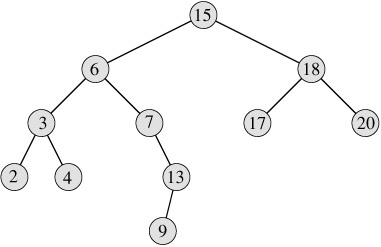
\includegraphics[scale=0.5]{img/tree.eps}
        \caption{example tree} \label{fig:example-tree}
       \end{center}
\end{figure}

\subsubsection*{C++ in-order walk testing and it's result.}

Suppose we have a pointer point to the tree contains data in figure 
\ref{fig:example-tree}. It can be created by build\_tree() function.

\lstset{language=C++}
\begin{lstlisting}
  struct Print{
    template<class T>
    void operator()(T x){ std::cout<<x<<", "; }
  };

  //...
  std::cout<<"test in order walk with print functor: ";
  in_order_walk(tree, Print());
\end{lstlisting}

In the above example, I created a function object Print, and pass an
instance of it to in-order walk process, it will print all the node
from less to greater with ',' as deliminator.

\begin{verbatim}
test in order walk with print functor: 2, 3, 4, 6, 7, 9, 13, 15, 
17, 18, 20,
\end{verbatim}

If boost::lambda is used, the above test cases can be simplied
a lot.
\begin{lstlisting}
//#include <boost/lambda/lambda.hpp> at the begin
using namespace boost::lambda;
std::cout<<"test in order walk with print functor: ";
in_order_walk(tree, std::cout<<_1<<", ");
\end{lstlisting}

While the Haskell version can be tested as below:

\lstset{language=Haskell}
\begin{lstlisting}
testTreeWalk = "test tree in-order walk by apply (-):\t"++
               show (inOrderWalk t2 (\x -> -x))

main = do
  putStrLn testTreeWalk
\end{lstlisting}

This test example 'maps' each keys in the tree to its negative value,
so it can output a result as below:

\begin{verbatim}
test tree in-order walk by apply (-):   Node (Node (Node 
(Node Empty (-2) Empty) (-3) (Node Empty (-4) Empty)) (-6) 
(Node Empty (-7) (Node (Node Empty (-9) Empty) (-13) 
Empty))) (-15) (Node (Node Empty (-17) Empty) (-18) (Node 
Empty (-20) Empty))
\end{verbatim}

While for Python, because Lambda expression mustn't be statement,
I defined a function print to apply to in-order walk for testing.

\lstset{language=Python}
\begin{lstlisting}
def my_print(x):
    print x

class Test:
    #...
    def test_in_order_walk(self):
        print "test in order walk with my_print: "
        in_order_walk(self.tree, my_print)
\end{lstlisting}

The result is:

\begin{verbatim}
test in order walk with my_print:
2
3
4
6
7
9
13
15
17
18
20
\end{verbatim}

The Scheme/Lisp version testing is similar to Haskell very much as below.

\lstset{language=lisp}
\begin{lstlisting}
(define (test-in-order-walk)
  (in-order-walk t1 (lambda (x) (- 0 x))))
\end{lstlisting}

The result is:

\begin{verbatim}
(test-in-order-walk)
;Value 11: ((((() -2 ()) -3 (() -4 ())) -6 (() -7 ((() -9 ()) 
-13 ()))) -15 ((() -17 ()) -18 (() -20 ())))
\end{verbatim}

TODO: add a exercise that given a pre-order traverse result and an in-order
traverse result, please write the post-order traverse result. (re-construct
the tree).

Exercise 2: Prove why in-order walk output the elements stored in a binary
search tree in increase order?


% ================================================================
% Querying a binary search tree
% ================================================================
\section{Querying a binary search tree}

This section provides implementation of querying operations which are
described in 12.2 of CLRS\cite{CLRS}

\subsection{Searching}
In CLRS\cite{CLRS}, searching is demonstrated in both recursive way and 
imperative way. According to the definition of binary search tree, search
a value in a tree can be realized in the following recursive manner.

\begin{itemize}
\item If the tree is empty, just return empty (not-found);
\item If the key of the root is equal to the value to be found, 
return the root;
\item If the value is less than the key of the root, search in the left
child.
\item Else, which means that the value is greater than the key of the 
root, search in the right child.
\end{itemize}

\subsubsection*{Haskell search implementation, recursive}
\lstset{language=Haskell}
\begin{lstlisting}
search::(Ord a)=> Tree a -> a -> Tree a
search Empty _ = Empty
search t x | key(t)==x = t
           | x < key(t) = search (left t) x
           | otherwise = search (right t) x
\end{lstlisting}

Haskell program of search is just translate the above recursive algorithm
description into code. Since it uses less than operator '<', the type
of the key value must be comparable. So the type variable is an instance 
of Ord type class.

\subsubsection*{C++ search implementation, imperative}
\lstset{language=C++}
\begin{lstlisting}
template<class T>
node<T>* search(node<T>* t, T x){
  while(t && t->value!=x){
    if(x < t->value) t=t->left;
    else t=t->right;
  }
  return t;
}
\end{lstlisting}

Search can also be implemented in an imperative way by replace the current
node to left child if the value to be search less than the key or to right 
child if greater than.

\subsubsection*{Python search implementation, imperative}
\lstset{language=Python}
\begin{lstlisting}
def tree_search(t, x):
    while(t!=None and t.key != x):
        if(x < t.key): t = t.left
        else: t = t.right
    return t
\end{lstlisting}

\subsubsection*{Scheme/Lisp search implementation, recursive}
\lstset{language=lisp}
\begin{lstlisting}
(define (tree-search tree x)
  (cond ((null? tree) tree)
	((equal? x (key tree)) tree)
	((< x (key tree)) (tree-search (left tree) x))
	(else (tree-search (right tree) x))))
\end{lstlisting}

To test search programs, for C++, I defined a special version of assert, named
as assert\_(), it can write logs to stdout to tell if the test case ok or fail.

here is C++ version of search testing.

\lstset{language=c++}
\begin{lstlisting}
template<class T> void assert_(std::string msg, T x, T y){
  std::cout<<msg;
  if(x==y)
    std::cout<<x<<" OK.\n";
  else
    std::cout<<x<<"!="<<y<<" Fail.\n";
}

node<int>* empty(0);
assert_("search empty: ", search(empty, 3), empty);
std::cout<<"search exist value: "
         <<tree_to_str(search(tree, 18))<<"\n";
assert_("search non-exist: ", search(tree, 5), empty);
\end{lstlisting}

The variable tree is created as describe in above section. This test example 
gives the result as.
\begin{verbatim}
search empty: 0 OK.
search exist value: ((empty), 17, (empty)), 18, ((empty), 20, (empty))
search non-exist: 0 OK.
\end{verbatim}

Next is Haskell version of search testing.

\lstset{language=Haskell}
\begin{lstlisting}
testSearch = "\ntest search empty tree:\t"++ show (search 
                     (Empty::Tree Int) 3) ++
             "\ntest search non exist node in tree:\t"++ 
                     show (search t2 5)++
             "\ntest search a node in tree:\t"++ show 
                     (search t2 18)

main = do
  putStrLn testSearch
\end{lstlisting}

Where t2 is defined as the example tree, the result is:
\begin{verbatim}
test search empty tree: Empty
test search non exist node in tree:     Empty
test search a node in tree:     Node (Node Empty 17 Empty) 
18 (Node Empty 20 Empty)
\end{verbatim}

For python, I also defined the helper assert function to output the test
result.

\lstset{language=Python}
\begin{lstlisting}
class Test:
    # ...
    def __assert(self, msg, x, y):
        if(x == y): msg = msg + "OK."
        else: msg = msg + str(x) + "!=" + str(y) + "Fail."
        print msg

    def test_search(self):
        self.__assert("search empty: ", 
                      tree_search(None, 3), None)
        print tree_to_str(tree_search(self.tree, 18))
        self.__assert("search non-exist: ", 
                      tree_search(self.tree, 5), None)
\end{lstlisting}

By calling the test\_search(), it will generate a result as same as the one
in C++.

For Scheme, the test cases are list like this:

\lstset{language=lisp}
\begin{lstlisting}
(define (test-search)
  (display (tree-search '() 3)) (newline)
  (display (tree-search t1 5)) (newline)
  (display (tree-search t1 18)))
\end{lstlisting}

And the results in evaluator gives:

\begin{verbatim}
(test-search)
()
()
((() 17 ()) 18 (() 20 ()))
;Unspecified return value
\end{verbatim}

\subsection{Minimum and maximum}

Minimum and maximum can be implemented from the property of binary search
tree, less keys are always in left child, and greater keys are in right.

For minimum, we can continue traverse the left sub tree until it is empty.
While for maximum, we traverse the right.

\subsubsection*{C++ version of max/min, imperative}

\lstset{language=c++}
\begin{lstlisting}
template<class T>
node<T>* min(node<T>* x){
  while(x && x->left)
    x = x->left;
  return x;
}

template<class T>
node<T>* max(node<T>* x){
  while(x && x->right)
    x = x->right;
  return x;
}
\end{lstlisting}

While in Haskell, in order not to conflict with the max/min functions 
defined in prelude, I change the name to maxt/mint.

\subsubsection*{Haskell version of max/min, recursive}
\lstset{language=Haskell}
\begin{lstlisting}
mint::Tree a -> Tree a
mint t = if isEmpty (left t) then t else mint (left t)

maxt::Tree a -> Tree a
maxt t = if isEmpty (right t) then t else maxt (right t)
\end{lstlisting}

In Python and Scheme/Lisp, I also renamed the functions to avoid
conflict with predefined max/min.

\subsubsection*{Python version of max/min, imperative}
\lstset{language=Python}
\begin{lstlisting}
def tree_min(t):
    while(t!=None and t.left != None):
        t = t.left
    return t

def tree_max(t):
    while(t!=None and t.right != None):
        t = t.right
    return t
\end{lstlisting}

\subsubsection*{Scheme/Lisp version of max/min, recursive}
\lstset{language=lisp}
\begin{lstlisting}
(define (tree-min tree)
  (if (null? (left tree))
      tree
      (tree-min (left tree))))

(define (tree-max tree)
  (if (null? (right tree))
      tree
      (tree-max (right tree))))
\end{lstlisting}

\subsubsection*{test case and result in C++}
\lstset{language=c++}
\begin{lstlisting}
node<int>* empty(0);
assert_("min(empty)=", min(empty), empty);
assert_("min(tree)=", min(tree)->value, 2);
assert_("max(empty)=",max(empty), empty);
assert_("max(tree)=", max(tree)->value, 20);
\end{lstlisting}

\begin{verbatim}
min(tree)=2 OK.
max(empty)=0 OK.
max(tree)=20 OK.
search empty: 0 OK.
\end{verbatim}

\subsubsection*{test case and result in Haskell}

\lstset{language=Haskell}
\begin{lstlisting}
testMinMax = "\ntest min empty:\t" ++ 
               (show (mint (Empty::Tree Int))) ++
             "\ntest min tree:\t" ++ show (mint t2) ++ 
             "\ntest max empty:\t" ++ 
               (show (maxt (Empty::Tree Int))) ++
             "\ntest max tree:\t" ++ show (maxt t2)

main = do
    putStrLn testMinMax
\end{lstlisting}

\begin{verbatim}
test min empty: Empty
test min tree:  Node Empty 2 Empty
test max empty: Empty
test max tree:  Node Empty 20 Empty
\end{verbatim}

\subsubsection*{test case and result in Python}

\lstset{language=Python}
\begin{lstlisting}
def test_min_max(self):
    self.__assert("min(empty): ", tree_min(None), None)
    self.__assert("min(tree): ", tree_min(self.tree).key, 2)
    self.__assert("max(empty): ", tree_max(None), None)
    self.__assert("max(tree): ", tree_max(self.tree).key, 20)
\end{lstlisting}

The output result is as same as the one in C++.

\subsubsection*{test case and result in Scheme/Lisp}

\lstset{language=lisp}
\begin{lstlisting}
(define (test-min-max)
  (display (tree-min '())) (newline)
  (display (tree-min t1)) (newline)
  (display (tree-max '())) (newline)
  (display (tree-max t1)))
\end{lstlisting}

\begin{verbatim}
(test-min-max)
()
(() 2 ())
()
(() 20 ())
;Unspecified return value
\end{verbatim}

\subsection{Successor and predecessor}

Successor and predecessor is useful when a tree is treated as a generic container,
and traversed by using iterator. It will be relative easier to implement if parent of
a node can be accessed directly. The C++ version and python version benefit from
this reason.

\subsubsection*{C++ version of succ/pred, imperative}

\lstset{language=C++}
\begin{lstlisting}
template<class T>
node<T>* succ(node<T>* x){
  if(x){
    if(x->right) return min(x->right);
    //find an ancestor, whose left child contains x
    node<T>* p = x->parent;
    while(p && p->right==x){
      x = p;
      p = p->parent;
    }
    return p;
  }
  return 0;
}

template<class T>
node<T>* pred(node<T>* x){
  if(x){
    if(x->left) return max(x->left);
    //find an ancestor, whose right child contains x
    node<T>* p = x->parent;
    while(p && p->left==x){
      x = p;
      p = p->parent;
    }
    return p;
  }
  return 0;
}
\end{lstlisting}

In function succ(), it takes a node in a tree, and tries to find the successor
of this node. if the node to be found is empty, it just returns it.

If the node has non-empty right child, the answer will be the min node in right
sub tree. While if it hasn't right sub tree, we must back track the ancestors 
of this node, try to find one, whose key is bigger. This can be approached 
by testing if the left child of an ancestor contains our node.

We can test the above program as below:

\begin{lstlisting}
assert_("succ 7: ", succ(search(tree, 7))->value, 9);
assert_("succ 13: ", succ(search(tree, 13))->value, 15);
assert_("succ 20: ", succ(search(tree, 20)), empty);
assert_("pred 6: ", pred(search(tree, 6))->value, 4);
assert_("pred 7: ", pred(search(tree, 7))->value, 6);
assert_("pred 2: ", pred(search(tree, 2)), empty);
\end{lstlisting}

And the result is:
\begin{verbatim}
succ 7: 9 OK.
succ 13: 15 OK.
succ 20: 0 OK.
pred 6: 4 OK.
pred 7: 6 OK.
pred 2: 0 OK.
\end{verbatim}

\subsubsection*{Haskell version of succ/pred, recursive}

In Haskell implementation, since I don't record parent for a node, it's hard
to find successor and predecessor in a easy way. I am not able to find a high
efficient way to realize them.

I defined some helper functions to find parent of a node in the tree, and filter
out the ancestor of a node which satisfies a predication. 

\lstset{language=Haskell}
\begin{lstlisting}
-- Find parent of a value in tree
-- The performance is low: O(h)
parent::(Ord a)=>Tree a -> a -> Tree a
parent Empty _ = Empty
parent t x | x < (key t) = if isParent (left t) x then t 
                              else parent (left t) x
           | x > (key t) = if isParent (right t) x then t 
                              else parent (right t) x
           | otherwise = Empty where
               isParent Empty _ = False
               isParent t x = (key t)==x

-- Find an ancestor of a value wich match a certain rule
-- Performance is very low.
findAncestor::(Ord a)=>Tree a -> a ->(a->a->Bool)-> Tree a
findAncestor t x f = checkParent t (parent t x) x f where
    checkParent _ Empty _ _ = Empty
    checkParent t p x f = if f (key p) x then p
                          else checkParent t (parent t (key p)) x f
\end{lstlisting}

The helper function, parent, takes 2 parameters, one is a tree, the other
is a value x. If the tree is empty, there is no parent, so the program returns
empty. In other case, it will test from root recursively to check if x is equal to
the key of the left sub tree root or right sub tree root.

The other helper function, findAncestor will utilize parent function. it takes 3
parameters, a tree, a value x, and a predicate function. the program will first 
check the direct parent of x matches the predicate. If succeeds, the parent will
be returned, else it will recursively check grand parent until finally reach to root.

With these 2 helpers, succ/pred can be realized as the following:
\begin{lstlisting}
-- Performance is very low.
succt::(Ord a)=>Tree a -> a -> Tree a
succt Empty _ = Empty
succt t x = if not (isEmpty rightNode)
            then mint rightNode
            else findAncestor t x (>) where
                rightNode = right (search t x)

-- Performance is very low
predt::(Ord a)=>Tree a -> a -> Tree a
predt Empty _ = Empty
predt t x = if not (isEmpty leftNode)
            then maxt leftNode
            else findAncestor t x (<) where
                leftNode = left (search t x)
\end{lstlisting}

For either cases, the program will fist call search function to locate the node
which key value is equal to x. In order to find the successor of a node, we'll 
check if the node has right child. If the right child isn't empty, the minimum 
of right sub tree is the answer, else we'll track back to find the nearest 
ancestor which is greater than x.

The test cases and result are as below:
\begin{lstlisting}
testSuccPred = 
  "\ntest succ of 7:\t"++ show (key (succt t2 7)) ++
  "\ntest succ of 13:\t"++ show (key (succt t2 13)) ++
  "\ntest pred of 6:\t"++ show (key (predt t2 6))++
  "\ntest pred of 7:\t"++ show (key (predt t2 7))

main = do
    putStrLn testSuccPred
    putStrLn testDel
\end{lstlisting}

\begin{verbatim}
test succ of 7: 9
test succ of 13:        15
test pred of 6: 4
test pred of 7: 6
\end{verbatim}

Note that there is a big problem in compute time of successor and predecessor 
operations if I implement them as above. For the imperative version, the time
is $O(h)$, where $h$ is the height of the tree ($h$ close to $log(N)$ if the
binary search tree is balanced), while it is quite slow than this because each
parent/ancestor finding operation takes $O(h)$ time. I am finding if there is 
better solution.

\subsubsection*{Python version of succ/pred, imperative}

Python version can be implemented very similar to C++ version. I changed it
a bit. When we seek for successor, in case a node hasn't right child, we have to find an ancestor of that
node, which has the node in ancestor's left sub tree. The change can be seen
in the while loop condition in below code.

\lstset{language=Python}
\begin{lstlisting}
def succ(x):
    if(x is None): return None
    if(x.right != None): return tree_min(x.right)
    p = x.parent
    while(p != None and p.left != x):
        x = p
        p = p.parent
    return p

def pred(x):
    if (x is None): return None
    if (x.left != None): return tree_max(x.left)
    p = x.parent
    while(p != None and p.right != x):
        x = p
        p = p.parent
    return p
\end{lstlisting}

The test cases for Python program are:
\begin{lstlisting}
def test_succ_pred(self):
    self.__assert("succ of 7: ", 
        succ(tree_search(self.tree, 7)).key, 9)
    self.__assert("succ of 13: ", 
        succ(tree_search(self.tree, 13)).key, 15)
    self.__assert("succ of 20: ", 
        succ(tree_search(self.tree, 20)), None)
    self.__assert("pred of 6: ", 
        pred(tree_search(self.tree, 6)).key, 4)
    self.__assert("pred of 7: ", 
        pred(tree_search(self.tree, 7)).key, 6)
    self.__assert("pred of 2: ", 
        pred(tree_search(self.tree, 2)), None)
\end{lstlisting}

The result is as same as the one output by C++ program.

\subsubsection*{Scheme/Lisp version of succ/pred, imperative}

\lstset{language=lisp}
\begin{lstlisting}
;; low efficiency functions
(define (parent tree x) ; x is a node, not a value
  (define (parent? t v)
    (if (null? t) t (equal? (key t) v)))
  (cond ((null? tree) tree)
	((< (key x) (key tree)) (if (parent? (left tree) (key x))
				    tree
				    (parent (left tree) x)))
	((> (key x) (key tree)) (if (parent? (right tree) (key x))
				    tree
				    (parent (right tree) x)))
	(else '())))

(define (find-ancestor tree x f) ; x is a node, not a value
  (define (check-parent t p v f)
    (if (f (key p) v)
	p
	(check-parent t (parent t p) v f)))
  (check-parent tree (parent tree x) (key x) f))

(define (succ tree x) ;x is a node, not a value
  (if (null? (right x))
      (find-ancestor tree x >)
      (tree-min (right x))))

(define (pred tree x)
  (if (null? (left x))
      (find-ancestor tree x <)
      (tree-max (left x))))
\end{lstlisting}

Similar to the Haskell version, Scheme version of succ/pred I wrote is poor
in term of performance. This is because there is no easy way to locate the
parent of a node. Anyone who finds a better version, please feel free to 
tell me.

The test cases and results are:

\begin{lstlisting}
(define (test-succ-pred)
  (display (key (succ t1 (tree-search t1 7)))) (newline)
  (display (key (succ t1 (tree-search t1 13)))) (newline)
  (display (key (pred t1 (tree-search t1 6)))) (newline)
  (display (key (pred t1 (tree-search t1 7)))))
\end{lstlisting}

\begin{verbatim}
(test-succ-pred)
9
15
4
6
;Unspecified return value
\end{verbatim}

% ================================================================
%                 Insertion and deletion
% ================================================================
\section{Insertion and deletion}

Different with all above tree operations, insertion and deletion can mutate
the tree. All functions I defined till now are 'read only' functions.

\subsection{Insertion}
Insertion is the necessary element to create a tree, one recursive description
of insertion is like this.

To insert a value x to a tree t,
\begin{itemize}
\item If the tree is empty, then return a leave with key=x;
\item If x is less than the key of root node, insert x to the left child;
\item If x is greater than the key of root, insert x to the right child.
\end{itemize}

\subsubsection*{Haskell tree insertion, recursive}
By translate the above description into Haskell code, the program can be written
as below.

\begin{lstlisting}
insert::(Ord a) => Tree a -> a -> Tree a
insert Empty x = leaf x
insert t x = if x < key(t) 
             then (Node (insert (left t) x) (key t) (right t))
             else (Node (left t) (key t) (insert (right t) x))
\end{lstlisting}

The testing of insertion can be found in section \ref{list2tree}

\subsubsection*{C++ tree insertion, imperative}

By using imperacitve language such as C++, we can iterate to the sub-tree untill
to the insertion point. There are some extra lines to set the parent of the node
properly.

\lstset{language=C++}
\begin{lstlisting}
template<class T>
node<T>* insert(node<T>* tree, T value){
  node<T>* root(tree);
  node<T>* x = new node<T>(value);
  node<T>* parent(0);
  while(tree){
    parent = tree;
    if(value < tree->value)
      tree = tree -> left;
    else //assert there is no duplicated value inserted.
      tree = tree -> right;
  }
  x->parent = parent;
  if( parent == 0 ) //tree is empty
    return x;
  else if( value < parent->value)
    parent->left = x;
  else
    parent->right = x;
  return root;
}
\end{lstlisting}

\subsubsection*{Python tree insertion, imperative}

\lstset{language=Python}
\begin{lstlisting}
def tree_insert(t, key):
    root = t
    x = Node(key)
    parent = None
    while(t):
        parent = t
        if(key < t.key):
            t = t.left
        else:
            t = t.right
    x.parent = parent
    if(parent == None): #tree is empty
        return x
    elif(key < parent.key):
        parent.left = x
    else:
        parent.right = x
    return root
\end{lstlisting}

\subsubsection*{Scheme/Lisp tree insertion, imperative}

\lstset{language=lisp}
\begin{lstlisting}
(define (tree-insert tree x)
  (cond ((null? tree) (list '() x '()))
	((< x (key tree))
	 (make-tree (tree-insert (left tree) x)
		    (key tree)
		    (right tree)))
	((> x (key tree))
	 (make-tree (left tree)
		    (key tree)
		    (tree-insert (right tree) x)))))
\end{lstlisting}

The testing can be refer to section \ref{list2tree}.

\subsection{Deletion}
Deletion is the most complex operation for binary search tree. this is because we
must keep the property, that left sub tree < key < right sub tree. Deleting a node
can break this property very easy.

I don't use the same algorithm described in CLRS\cite{CLRS}, I found a more simple
one from 'Annotated STL'\cite{hj-stl}

The algorithm can be described as below:

To delete a node x from a tree.
\begin{itemize}
\item If x has no child or only one child, splice x out;
\item If x has two children, use minimum of its right to replace x, 
and splice the original minimum out.
\end{itemize}

\subsubsection*{Haskell deletion, recursive}

Haskell version of deletion can be realized by translating the above description
directly into code. But there is a different point, instead of pass a node to the
function, I pass value to be deleted in it. So the program need perform search first.

\lstset{language=Haskell}
\begin{lstlisting}
delete::(Ord a)=> Tree a -> a -> Tree a
delete Empty _ = Empty
delete (Node l k r) x | x < k = (Node (delete l x) k r)
                      | x > k = (Node l k (delete r x))
                      -- x == k
                      | isEmpty l = r
                      | isEmpty r = l
                      | otherwise = (Node l k' (delete r k')) 
                          where k' = key (mint r)
\end{lstlisting}

The test cases and result are shows as below.

\begin{lstlisting}
testDel = "\ntest del 17:\t"++ show (delete t2 17)++
          "\ntest del 7:\t"++ show (delete t2 7)++
          "\ntest del 6:\t" ++ show (delete t2 6)++
          "\ntest del 15:\t"++ show (delete t2 15)++
          "\ntest del non-exist:\t" ++ show (delete t2 5)

main = do
    putStrLn testDel
\end{lstlisting}

\begin{verbatim}
test del 17:    Node (Node (Node (Node Empty 2 Empty) 3 (Node Empty 4 
Empty)) 6 (Node Empty 7 (Node (Node Empty 9 Empty) 13 Empty))) 15 
(Node Empty 18 (Node Empty 20 Empty))
test del 7:     Node (Node (Node (Node Empty 2 Empty) 3 (Node Empty 4 
Empty)) 6 (Node (Node Empty 9 Empty) 13 Empty)) 15 (Node (Node Empty 
17 Empty) 18 (Node Empty 20 Empty))
test del 6:     Node (Node (Node (Node Empty 2 Empty) 3 (Node Empty 4 
Empty)) 7 (Node (Node Empty 9 Empty) 13 Empty)) 15 (Node (Node Empty 
17 Empty) 18 (Node Empty 20 Empty))
test del 15:    Node (Node (Node (Node Empty 2 Empty) 3 (Node Empty 4 
Empty)) 6 (Node Empty 7 (Node (Node Empty 9 Empty) 13 Empty))) 17 
(Node Empty 18 (Node Empty 20 Empty))
test del non-exist:     Node (Node (Node (Node Empty 2 Empty) 3 (Node 
Empty 4 Empty)) 6 (Node Empty 7 (Node (Node Empty 9 Empty) 13 Empty))) 
15 (Node (Node Empty 17 Empty) 18 (Node Empty 20 Empty))
\end{verbatim}

\subsubsection*{C++ deletion, imperative}

C++ version is more complex because it need set the parent properly.
While we can pass the pointer to the node which will be deleted to the function,
so that search is no more needed. The function will return the root
of the result tree.

\lstset{language=C++}
\begin{lstlisting}
template<class T>
node<T>* del(node<T>* tree, node<T>* x){
  if(!x)
    return tree;

  node<T>* root(tree);
  node<T>* old_x(x);
  node<T>* parent(x->parent);

  if(x->left == 0)
    x = x->right;
  else if(x->right == 0)
    x = x->left;
  else{
    node<T>* y=min(x->right);
    x->value = y->value;
    if(y->parent != x)
      y->parent->left = y->right;
    else
      x->right = y->right;

    remove_node(y);
    return root;
  }

  if(x)
    x->parent = parent;

  if(!parent)
    root = x; //remove node of a tree
  else
    if(parent->left == old_x)
      parent->left = x;
    else
      parent->right = x;

  remove_node(old_x);
  return root;
}
\end{lstlisting}

If the node to be deleted is empty, the function simply returns the original tree.
In other cases, it will first record the root of the tree, create a copy pointer
to x, and to its parent.

If either of the children is empty, the program just splice x out. If it has two
none-empty children, we first located the minimum of right child, replace the key
of x to y's, then splice y out. Note that the helper function remove\_node() is
used.

Finally we reset the parent. If the parent pointer we copied before is empty, it
means that we are deleting the root node, so we need return the new root. After
the parent is set properly, we finally remove the old x from memory.

The test cases and result are shows as below.

\begin{lstlisting}
void test_del_n(int n){
  node<int>* empty(0);
  node<int>* t1=clone_tree(tree);
  t1=del(t1, search(t1, n));
  std::cout<<"del "<<n<<":\n"<<tree_to_str(t1)<<"\n";
  assert_("search after del: ", search(t1, n), empty);
  delete t1;
}

test_del_n(17);
test_del_n(7);
test_del_n(6);
test_del_n(15);
test_del_n(1); //try to del a non-exist val
\end{lstlisting}

Because the deletion function in C++ inplace change the tree, so I cloned the test 
tree for each testing. The clone\_tree() function is defined in section \ref{helper-fun}.

The result of these test case is as below.
\begin{verbatim}
del 17:
((((empty), 2, (empty)), 3, ((empty), 4, (empty))), 6, ((empty), 7, 
(((empty), 9, (empty)), 13, (empty)))), 15, ((empty), 18, ((empty), 
20, (empty)))
search after del: 0 OK.
del 7:
((((empty), 2, (empty)), 3, ((empty), 4, (empty))), 6, (((empty), 9, 
(empty)), 13, (empty))), 15, (((empty), 17, (empty)), 18, ((empty), 
20, (empty)))
search after del: 0 OK.
del 6:
((((empty), 2, (empty)), 3, ((empty), 4, (empty))), 7, (((empty), 9, 
(empty)), 13, (empty))), 15, (((empty), 17, (empty)), 18, ((empty), 
20, (empty)))
search after del: 0 OK.
del 15:
((((empty), 2, (empty)), 3, ((empty), 4, (empty))), 6, ((empty), 7, 
(((empty), 9, (empty)), 13, (empty)))), 17, ((empty), 18, ((empty), 
20, (empty)))
search after del: 0 OK.
del 1:
((((empty), 2, (empty)), 3, ((empty), 4, (empty))), 6, ((empty), 7, 
(((empty), 9, (empty)), 13, (empty)))), 15, (((empty), 17, (empty)), 
18, ((empty), 20, (empty)))
search after del: 0 OK.
\end{verbatim}

\subsubsection*{Python deletion, imperative}
Python version is very similar to C++, but it needn't free memory because
of GC support.

\lstset{language=Python}
\begin{lstlisting}
def tree_delete(t, x):
    if (x is None): return t
    [root, old_x, parent] = [t, x, x.parent]
    if (x.left is None):
        x = x.right
    elif (x.right is None):
        x = x.left
    else:
        y = tree_min(x.right)
        x.key = y.key
        if (y.parent != x):
            y.parent.left = y.right
        else:
            x.right = y.right
        remove_node(y)
        return root
    if (x != None):
        x.parent = parent
    if (parent != None):
        root = x
    else:
        if(parent.left == old_x): parent.left = x
        else: parent.right = x
    remove_node(old_x)
    return root
\end{lstlisting}

This function can be tested as below:

\begin{lstlisting}
def __test_del_n(self, n):
    t = clone_tree(self.tree)
    t = tree_delete(t, tree_search(t, n))
    print "del ", n, ": ", tree_to_str(t)
    self.__assert("search after del: ", tree_search(t, n), None)

def test_del(self):
    self.__test_del_n(17)
    self.__test_del_n(7)
    self.__test_del_n(6)
    self.__test_del_n(15)
    self.__test_del_n(1) #del a non-exist value
\end{lstlisting}

The test result is as same as C++.

\subsubsection*{Scheme/Lisp deletion, recursive}

\lstset{language=lisp}
\begin{lstlisting}
(define (tree-delete tree v)
  (cond ((null? tree) tree)
	((< v (key tree)) (make-tree (tree-delete (left tree) v)
				     (key tree)
				     (right tree)))
	((> v (key tree)) (make-tree (left tree)
				     (key tree)
				     (tree-delete (right tree) v)))
	((null? (left tree)) (right tree))
	((null? (right tree)) (left tree))
	(else (let ((newkey (key (tree-min (right tree)))))
		(make-tree (left tree)
			   newkey
			   (tree-delete (right tree) newkey))))))
\end{lstlisting}

Test cases are like the following.

\begin{lstlisting}
(define (test-del)
  (display (tree-delete t1 17)) (newline)
  (display (tree-delete t1 7)) (newline)
  (display (tree-delete t1 6)) (newline)
  (display (tree-delete t1 15)) (newline)
  (display (tree-delete t1 5)))
\end{lstlisting}

It will output the result in emulator as below.

\begin{verbatim}
(test-del)
((((() 2 ()) 3 (() 4 ())) 6 (() 7 ((() 9 ()) 13 ()))) 15 (() 18 (() 20 ())))
((((() 2 ()) 3 (() 4 ())) 6 ((() 9 ()) 13 ())) 15 ((() 17 ()) 18 (() 20 ())))
((((() 2 ()) 3 (() 4 ())) 7 ((() 9 ()) 13 ())) 15 ((() 17 ()) 18 (() 20 ())))
((((() 2 ()) 3 (() 4 ())) 6 (() 7 ((() 9 ()) 13 ()))) 17 (() 18 (() 20 ())))
((((() 2 ()) 3 (() 4 ())) 6 (() 7 ((() 9 ()) 13 ()))) 15 ((() 17 ()) 18 (() 
20 ())))
;Unspecified return value
\end{verbatim}

\section{Randomly built binary search tree}
In CRLS\cite{CLRS}, it described about randomly built binary search tree.
Ramdomly building can help to avoid (decrease the possibility) unbalanced
binary trees.

This can be easily implemented in imperative way, such as by C++ and Python.
Before call build\_tree() or list\_to\_tree() function, we can call random
process, to shuffle the list or collection. The same approach can also be
used in Scheme/Lisp. While for pure functional programming language, such as
Haskell, randomization violate the property of pure function. We have to
use alternative approach such as Monad.

There are more solution to ensure the tree is balanced, such as red black tree,
please refer to other posts for detailed implementation.

\section{Appendix} \label{appendix}
%\appendix
All programs are provided along with this article. They are free for downloading.
\begin{itemize}
\item bstree.cpp, C++ version of binary seach tree, including all test cases. I 
compiled and tested it with GUN G++ 3.4.4.
\item BSTree.hs, Haskell version of binary search tree, with test cases. I compiled
and tested it with GHC 6.10.4.
\item bstree.py, Python version of the binary search tree, with test cases. Tested
with Python 2.5.1
\item bstree.scm, Scheme version of the binary search tree and test cases. Tested
with MIT/Scheme 14.9
\end{itemize}
download position: http://sites.google.com/site/algoxy/bstree/bstree.zip

\begin{thebibliography}{99}

\bibitem{CLRS}
Thomas H. Cormen, Charles E. Leiserson, Ronald L. Rivest and Clifford Stein. 
``Introduction to Algorithms, Second Edition''. ISBN:0262032937. The MIT Press. 2001

\bibitem{Bentley}
Jon Bentley. ``Programming Pearls(2nd Edition)''. Addison-Wesley Professional; 2 edition (October 7, 1999). ISBN-13: 978-0201657883

\bibitem{hj-stl}
Hou Jie. ``The annotated STL sources (using SGI STL)''. ISBN:7-5609-2699-1 http://press.hust.edu.cn. 2002.

\bibitem{literal-program}
http://en.literateprograms.org/Category:Binary\_search\_tree

\bibitem{wiki-fold}
http://en.wikipedia.org/wiki/Foldl

\end{thebibliography}

\ifx\wholebook\relax\else
\end{document}
\fi
